\documentclass[b4paper, landscape, dvipdfmx]{jsarticle}
%----- 必要なパッケージ -----
\usepackage{fancybox,ascmac,otf}
\usepackage{amssymb, amsthm}
\usepackage[leqno]{amsmath}
\usepackage{geometry}
\usepackage{multicol}
\usepackage{tcolorbox}
\usepackage{xcolor}
\usepackage{fancyhdr}
\usepackage{tikz}

% TikZライブラリ
\usetikzlibrary{
    positioning,
    arrows.meta,
    calc,
    shadows,
    shadows.blur,
    intersections,
    angles,
    quotes,
    decorations.pathmorphing
}

% tcolorboxライブラリ
\tcbuselibrary{skins, breakable, theorems}

\usepackage{enumitem}
\setlist[enumerate,1]{label=(\arabic*)}
\setlist[itemize]{leftmargin=*}
\newcommand{\ds}{\displaystyle}

%----- レイアウト設定 -----
\geometry{
  left=15mm,
  right=15mm,
  top=20mm,
  bottom=15mm,
  headheight=25pt
}

%----- 数式環境の上下の余白調整 -----
\AtBeginDocument{
  \setlength{\abovedisplayskip}{5pt}
  \setlength{\belowdisplayskip}{5pt}
  \setlength{\abovedisplayshortskip}{0pt}
  \setlength{\belowdisplayshortskip}{3pt}
}

%===========================================================
%  デザイン設定
%===========================================================

%--- 色の定義 ---
\definecolor{printBlue}{RGB}{0, 50, 100}     % 濃紺
\definecolor{printRed}{RGB}{140, 20, 20}     % 濃エンジ
\definecolor{printTeal}{RGB}{0, 60, 60}      % 濃い青緑

%--- 共通スタイル定義 ---
\tcbset{
    chartbox/.style={
        enhanced,
        fonttitle=\sffamily\bfseries,
        boxrule=1pt,
        arc=2pt,
        top=1.0em,
        nobeforeafter,
        enlarge left by=-2mm,
        enlarge right by=-2mm,
        drop fuzzy shadow,
        colback=white,
        attach boxed title to top left={xshift=10pt, yshift*=-\tcboxedtitleheight/2},
        boxed title style={frame hidden, sharp corners, rounded corners=southeast, arc=3pt}
    }
}

%--- 各種ボックス環境定義 ---
\newtcolorbox{any}[1]{
    enlarge left by=0mm, enlarge right by=0mm,
    enhanced, frame hidden, colback=white, title={#1},
    attach boxed title to top left={xshift=0mm, yshift=0mm},
    coltitle=white, fonttitle=\bfseries\sffamily,
    boxed title style={
        colback=black!80, frame hidden, arc=4pt, outer arc=4pt,
        sharp corners=south, boxrule=0pt,
        top=1mm, bottom=1mm, left=3mm, right=3mm
    },
    underlay boxed title={
        \draw[thick, black!80] (title.south west) -- (title.south west-|frame.east);
    },
    breakable, top=5mm, left=2mm, right=2mm, bottom=0mm,
    before skip=1em, after skip=1em,
    segmentation style={draw=black!40, dashed}
}

\newtcolorbox{eg}[1]{
    chartbox,
    colframe=printBlue,
    coltitle=white,
    title=\textbf{例題 #1},
    boxed title style={colback=printBlue},
    segmentation style={draw=printBlue, line width=0.5pt, dashed}
}

\newtcolorbox{prac}[1]{
    chartbox,
    colframe=printRed,
    coltitle=white,
    title=\textbf{練習 #1},
    boxed title style={colback=printRed}
}

\newtcolorbox{thm}[1]{
    chartbox,
    colframe=printTeal,
    coltitle=white,
    title=\textbf{#1},
    boxed title style={colback=printTeal}
}

\newtcolorbox{answer}[1][height fill]{
    enhanced,
    title={Memo / Answer},
    colframe=black!80,
    colback=white,
    coltitle=black!60,
    fonttitle=\sffamily\bfseries,
    attach boxed title to top left={xshift=5mm, yshift*=-\tcboxedtitleheight/2},
    boxed title style={frame hidden, colback=white},
    boxrule=1pt,
    arc=1pt,
    nobeforeafter,
    enlarge left by=-2mm, 
    enlarge right by=-2mm, 
    height fill,
    segmentation style={draw=black!20, solid},
    underlay={
        \begin{tcbclipinterior}
            \draw[step=5mm, black!5, ultra thin] (interior.south west) grid (interior.north east);
        \end{tcbclipinterior}
    }, 
    #1
}

%----- ヘッダーの設定 -----
\pagestyle{fancy}
\fancyhf{}
\fancyhead[C]{%
    \begin{tikzpicture}[remember picture, overlay]
        \node[anchor=north west, fill=printBlue, minimum width=\paperwidth, minimum height=5pt] at (current page.north west) {};
    \end{tikzpicture}
}
\fancyhead[L]{\small \textcolor{black!90}{数学C $>$ 第1章--平面ベクトル $>$ 第9回 \textbf{交点の位置ベクトル}}}
\fancyhead[R]{\small 年 \hspace{1cm} 組 \hspace{1cm} 番 \quad 氏名 \hspace{6cm}}
\renewcommand{\headrulewidth}{0pt}

\begin{document}

%=============================================================================
% 1枚目:交点の解法(基本)
%=============================================================================
\begin{multicols}{2}

%-----------------------------------------------------------------------------
% 左カラム:2通りで表して係数比較
%-----------------------------------------------------------------------------
\begin{any}{1. 交点の定番解法(2通りで表す)}
    2直線 AD, BC の交点 P の位置ベクトルを求める問題は, ベクトルで最も重要なパターンの1つである.
    \textbf{「Pは直線AD上にある」}かつ\textbf{「Pは直線BC上にある」}という2つの情報を数式にして連立する.

    \begin{eg}{1 (交点の位置ベクトル)}
        $\triangle$OAB において, 辺 OA を $5:2$ に内分する点を C, 辺 OB を $2:1$ に内分する点を D とする.
        線分 AD と BC の交点を P とし, $\overrightarrow{\text{OA}}=\vec{a}, \overrightarrow{\text{OB}}=\vec{b}$ とする.
        $\overrightarrow{\text{OP}}$ を $\vec{a}, \vec{b}$ で表せ.
        
        \tcblower
        \begin{center}
        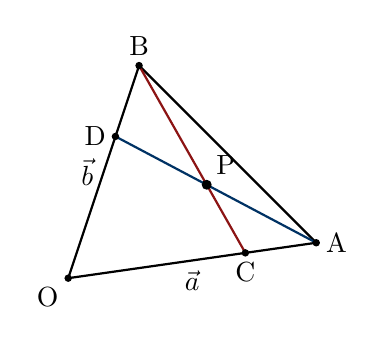
\begin{tikzpicture}[scale=0.9]
            \coordinate (O) at (0,0);
            \coordinate (A) at (3.5, 0.5);
            \coordinate (B) at (1, 3);
            
            % C is on OA (5:2) -> 5/7 of OA
            \coordinate (C) at ($ (O)!5/7!(A) $);
            % D is on OB (2:1) -> 2/3 of OB
            \coordinate (D) at ($ (O)!2/3!(B) $);
            
            % Intersection P
            \path[name path=lineAD] (A) -- (D);
            \path[name path=lineBC] (B) -- (C);
            \path[name intersections={of=lineAD and lineBC, by=P}];
            
            \draw[thick] (O)--(A) node[midway, below] {$\vec{a}$};
            \draw[thick] (O)--(B) node[midway, left] {$\vec{b}$};
            \draw[thick] (A)--(B);
            \draw[thick, printBlue] (A)--(D);
            \draw[thick, printRed] (B)--(C);
            
            \fill (O) circle (1.5pt) node[below left] {O};
            \fill (A) circle (1.5pt) node[right] {A};
            \fill (B) circle (1.5pt) node[above] {B};
            \fill (C) circle (1.5pt) node[below] {C};
            \fill (D) circle (1.5pt) node[left] {D};
            \fill (P) circle (2pt) node[above right] {P};
        \end{tikzpicture}
        \end{center}
        \vspace{10cm} % 解答スペース
    \end{eg}
    
    % \textbf{解法のアルゴリズム:}
    % \begin{enumerate}
    %     \item 点Pを「線分AD上の点」として, $(1-s)\vec{a} + s\vec{d}$ と表す.
    %     \item 点Pを「線分BC上の点」として, $(1-t)\overrightarrow{\text{OC}} + t\vec{b}$ と表す.
    %     \item 係数を比較して連立方程式を解く.
    % \end{enumerate}
\end{any}

%-----------------------------------------------------------------------------
% 右カラム:幾何的な別解(検算)
%-----------------------------------------------------------------------------
\columnbreak

\begin{any}{2. メネラウスの定理(検算の魔法)}
    記述試験では係数比較(左の解法)を書くべきだが, 答えだけ求めたい場合や検算には\textbf{図形の性質}を使うと圧倒的に速い.

   \begin{thm}{メネラウスの定理}
        \begin{minipage}{0.55\linewidth}
            右図のような形(キツネ型)において, 一筆書きの要領で比を掛けると1になる.
            \[ \frac{CE}{EB} \times \frac{BD}{DA} \times \frac{AF}{FC} = 1 \]
            \small{※頂点$\to$分点$\to$頂点...と回る}
        \end{minipage}
        \hfill
        \begin{minipage}{0.40\linewidth}
            \centering
            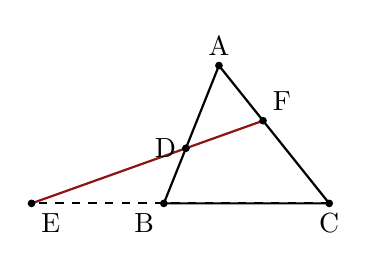
\begin{tikzpicture}[scale=0.7, >=stealth]
                % 座標定義
                \coordinate (A) at (1, 2.5);
                \coordinate (B) at (0, 0);
                \coordinate (C) at (3, 0);
                
                % 分点定義
                \coordinate (D) at ($(A)!0.6!(B)$); % AB上の点
                \coordinate (F) at ($(A)!0.4!(C)$); % AC上の点
                
                % 交点E (BCの延長とDFの交点)
                \coordinate (E) at (intersection of B--C and D--F);
                
                % 三角形と直線の描画
                \draw[thick] (A) -- (B) -- (C) -- cycle;
                \draw[thick, dashed] (C) -- (E); % 延長部分
                \draw[thick, printRed] (F) -- (E); % 串刺し線(キツネの目)
                
                % 点の描画
                \fill (A) circle (2pt) node[above] {A};
                \fill (B) circle (2pt) node[below left] {B};
                \fill (C) circle (2pt) node[below] {C};
                \fill (D) circle (2pt) node[left] {D};
                \fill (E) circle (2pt) node[below right] {E};
                \fill (F) circle (2pt) node[above right] {F};
            \end{tikzpicture}
        \end{minipage}
    \end{thm}

    \begin{eg}{2 (比の計算と検算)}
        例題1について, メネラウスの定理を用いて $AP:PD$ および $BP:PC$ を求めよ.
        また, その比を用いて $\overrightarrow{\text{OP}}$ を求め, 例題1の答えと一致するか確認せよ.
        
        \tcblower
        \vspace{10cm}
    \end{eg}
\end{any}

\end{multicols}

%=============================================================================
% 2枚目:確認テスト(問題)
%=============================================================================
\newpage
\fancyhead[L]{\small \textcolor{black!90}{数学C $>$ 第1章--平面ベクトル $>$ 第9回--\textbf{確認テスト}}}
\begin{multicols}{2}

\begin{any}{確認テスト (A: 基本)}
    \begin{prac}{A1 (交点の計算)}
        $\triangle$OAB において, 辺 OA の中点を C, 辺 OB を $1:2$ に内分する点を D とする.
        線分 AD と BC の交点を P とする.
        $\overrightarrow{\text{OA}}=\vec{a}, \overrightarrow{\text{OB}}=\vec{b}$ とするとき,
        $\overrightarrow{\text{OP}}$ を $\vec{a}, \vec{b}$ で表せ.
    \end{prac}
    \begin{answer}[height=8cm]
    \end{answer}
\end{any}

\columnbreak

\begin{any}{確認テスト (B: 標準)}
    \begin{prac}{B1 (面積比)}
       練習A1の設定において, 以下の線分の比を求めよ.
        \begin{enumerate}
            \item $AP : PD$
            \item $BP : PC$
        \end{enumerate}
    \end{prac}
    \begin{answer}[height=6cm]
    \end{answer}

    \begin{prac}{B2 (一直線上の点)}
        $\triangle$OAB において, $\overrightarrow{\text{OA}}=\vec{a}, \overrightarrow{\text{OB}}=\vec{b}$ とする.
        $\overrightarrow{\text{OP}} = 3\vec{a} + 4\vec{b}$ であるとき, 直線 OP と線分 AB の交点 Q の位置ベクトル $\overrightarrow{\text{OQ}}$ を $\vec{a}, \vec{b}$ で表せ.
        \\
        (\textbf{ヒント:} QはOP上の点なので $\overrightarrow{\text{OQ}} = k\overrightarrow{\text{OP}}$. またQはAB上にあるので係数の和が...?)
    \end{prac}
    \begin{answer}[height=6cm]
    \end{answer}
\end{any}

\end{multicols}

%=============================================================================
% 3枚目:確認テスト(解答)
%=============================================================================
\newpage
\fancyhead[L]{\small \textcolor{black!90}{数学C $>$ 第1章--平面ベクトル $>$ 第9回 \textbf{【解答解説】}}}

\begin{multicols}{2}

\begin{any}{解答 A}
    \begin{answer}[height=8cm]
    \color{printRed}
    \textbf{A1 解答}:\\
        $\vec{c} = \frac{1}{2}\vec{a}, \vec{d} = \frac{1}{3}\vec{b}$.
        
        (1) PはAD上: $\vec{p} = (1-s)\vec{a} + s\vec{d} = (1-s)\vec{a} + \frac{1}{3}s\vec{b}$.
        (2) PはBC上: $\vec{p} = (1-t)\vec{c} + t\vec{b} = \frac{1}{2}(1-t)\vec{a} + t\vec{b}$.
        
        連立方程式:
        $1-s = \frac{1}{2}(1-t), \quad \frac{1}{3}s = t$.
        代入して $1-s = \frac{1}{2}(1-\frac{1}{3}s) \implies 2-2s = 1 - \frac{1}{3}s$.
        $1 = \frac{5}{3}s \implies s = \frac{3}{5}$.
        
        よって, $\vec{p} = (1-\frac{3}{5})\vec{a} + \frac{1}{3}\cdot\frac{3}{5}\vec{b} = \boldsymbol{\frac{2}{5}\vec{a} + \frac{1}{5}\vec{b}}$
    \end{answer}
\end{any}

\columnbreak

\begin{any}{解答 B}
    \begin{answer}[height=8cm]
    \color{printRed}
    A1 の計算過程を利用する.
        
        (1) $AP:PD$ \\
        Pは線分ADを $s : (1-s)$ に内分する点である.
        A1より $s = \frac{3}{5}$ なので,
        \[ AP : PD = s : (1-s) = \frac{3}{5} : \frac{2}{5} = \boldsymbol{3:2} \]
        
        (2) $BP:PC$ \\
        Pは線分BCを $t : (1-t)$ に内分する点である. \textbf{(注意: $\vec{b}$の係数が$t$)}
        $t = \frac{1}{3}s = \frac{1}{3} \cdot \frac{3}{5} = \frac{1}{5}$.
        CからBへ向かうベクトルで考えたとき, C側の比率が $t$.
        つまり $CP : PB = t : (1-t) = 1 : 4$.
        あるいは $\vec{p} = (1-t)\vec{c} + t\vec{b}$ の係数を見て,
        $BP : PC = (1-t) : t = \frac{4}{5} : \frac{1}{5} = \boldsymbol{4:1}$.
    \end{answer}

    \begin{answer}[height=6cm]
    \color{printRed}
    \textbf{B2 解答}:\\
        QはOP上にあるので, $\overrightarrow{\text{OQ}} = k \overrightarrow{\text{OP}} = 3k\vec{a} + 4k\vec{b}$.
        QはAB上にあるので, 係数の和が 1.
        $3k + 4k = 1 \implies 7k = 1 \implies k = \frac{1}{7}$.
        
        よって,
        $\boldsymbol{\overrightarrow{\text{OQ}} = \frac{3}{7}\vec{a} + \frac{4}{7}\vec{b}}$
    \end{answer}
\end{any}

\end{multicols}
\end{document}